\documentclass{seal_thesis}

\thesisType{Bachelor Thesis}
\date{\today}
\title{Identifying flaky tests by classifiers}
\subtitle{A performance analysis of various machine learning models}
\author{Christian Birchler}
\home{Lucerne} % Geburtsort
\country{Switzerland}
\legi{15-924-160}
\prof{Prof. Dr. Harald C. Gall}
\assistent{Giovanni Grano\\Christoph Laaber}
\email{christian.birchler2@uzh.ch}
%\url{<url if available>}
\begindate{17. February 2020}
\enddate{17. August 2020}

\begin{document}
\maketitle

\frontmatter

\begin{acknowledgements}
First of all I would like to thank Giovanni Grano and Christoph Laaber for supervising me during my bachelor's thesis. You gave me valuable feedback on a weekly basis although we had to do the meetings virtually due to the COVID-19 pandemic. \\

\noindent Furthermore, I would like to thank Professor Gall for allowing me to do the thesis at his research group and to use the infrastructure on ScienceCloud. \\

\noindent I want also to thank my sister Alexandra Birchler for proofreading the thesis especially to improve the grammar and my writing. Last but not least I want to thank my friend Svenja Keller for giving motivation and insights of her master thesis.
\end{acknowledgements}

\begin{abstract}
Testing is a crucial part in software development. Most of the current bigger software projects integrate the testing in a continuous integration (CI) pipeline. A failing test will prevent the deployment of the software. In case of flaky tests where tests may fail and pass non-deterministically without a change to the code or the environment is an issue to deal with, since the developer is probably spending time to find a bug although the code under test is not defect. Previous studies focused mainly on the root causes of flakiness but only a few research was done on how to mitigate flaky tests. In this thesis we investigated the impact of different memory related JVM metrics on the predictability of flaky tests. For this purpose we took JVM metrics of 82 open-source Maven projects which had already recorded flaky tests. In order to take the measurements a toolchain script was developed, that injected the necessary code in to the test code so that JVM metrics could be collected during test executions. The toolchain ran for each project the test suites ten times to identify flaky tests that have different outcomes. The toolchain ran on different machines with different RAM sizes to see if there is a difference in the data. We did a PCA and a biplot to identify cluster structure in a lower dimensional space and applied various parametric and non-parametric classification models on the data. The results show that flaky tests are to a certain degree predictable by JVM metrics and the RAM size has also an impact on the predictability of flakiness. This insights allows to develop new tools to handle flaky tests and motivate more research.
\end{abstract}

\begin{zusammenfassung}
Testen ist ein entscheidender Bestandteil der Softwareentwicklung. Die meisten der derzeit größeren Softwareprojekte integrieren die Tests in eine CI-Pipeline (Continuous Integration). Ein fehlgeschlagener Test verhindert die Bereitstellung der Software. Bei Flaky-Tests, bei denen Tests fehlschlagen und nicht deterministisch ohne Änderung des Codes oder der Umgebung bestehen können, ist dies ein Problem, da der Entwickler wahrscheinlich Zeit damit verbringt, einen Fehler zu finden, obwohl der zu testende Code nicht fehlerhaft ist. Frühere Studien konzentrierten sich hauptsächlich auf die Ursachen von Flaky-Tests, es wurden jedoch nur wenige Untersuchungen durchgeführt, um Flaky-Tests zu erkennen. In dieser Arbeit untersuchten wir den Einfluss verschiedener speicherbezogener JVM-Metriken auf die Vorhersagbarkeit von Flaky-Tests. Zu diesem Zweck haben wir JVM-Metriken von 82 Open-Source-Maven-Projekten verwendet, die bereits Flaky-Tests aufgezeichnet hatten. Um die Messungen durchzuführen, wurde ein Toolchain-Skript entwickelt, das den erforderlichen Mess-Code in den Testcode einfügt, damit JVM-Metriken während der Testausführung erfasst werden können. Die Toolchain wurde für jedes Projekt zehn Mal ausgeführt, um Flaky-Tests mit unterschiedlichen Ergebnissen zu identifizieren. Die Toolchain wurde auf verschiedenen Computern mit unterschiedlichen RAM-Größen ausgeführt, um festzustellen, ob sich die Daten unterscheiden. Wir haben eine PCA und einen Biplot durchgeführt, um die Clusterstruktur in einem Raum mit niedrigeren Dimensionen zu identifizieren, und verschiedene parametrische und nicht parametrische Klassifizierungsmodelle auf die Daten angewendet. Die Ergebnisse zeigen, dass Flaky-Tests bis zu einem gewissen Grad durch JVM-Metriken vorhersagbar sind und die RAM-Größe auch einen Einfluss auf die Vorhersagbarkeit von Flaky-Tests hat. Diese Erkenntnisse ermöglichen es, neue Werkzeuge zu entwickeln, um Flaky-Tests zu handhaben und um für mehr Forschung von Flaky-Tests zu motivieren.
\end{zusammenfassung}

\tableofcontents
\listoffigures
\listoftables
\lstlistoflistings

\mainmatter
\chapter{Introduction}
Software testing is nowadays automated and embedded in a \textit{continous integration/delivery} (CI/CD) pipeline. Such automation makes it easier to bring the latest code changes into production. The production build usually relies on a passing test suite, which is a part of a CI/CD pipeline. Any unwanted interruptions in terms of failing tests will lead to a postponed deployment of the software and will produce more costs. Usually a failing test will indicate that in a certain module of the software is a defect, which must be resolved by the developers. But in case of so called \textit{flaky tests} a developer usually does not know if the defect lies in the test code itself or in the code under test \cite{daniel09}. Flaky tests are tests that have a non-deterministic behavior. Such tests pass and fail on different runs without any code changes. \\

\noindent The first intense study on flaky tests were done by \textit{Luo et al.} \cite{luo14}. They had the main goal to understand the root causes of flaky tests and presented a categorization of various causes of flakiness. In total they identfied 10 root causes (see table \ref{tab:luo14}). In addition to the first study \textit{Eck et al.} \cite{eck19} continued studying flaky tests but from a developer's perspective. They asked 21 professional developers to classify 200 flaky tests they previously fixed. One of the main insights was that they identified four more root causes for flakiness next to the root causes identified by \textit{Luo et. al}. There is also research on flaky tests for platform specific application like \textit{Android}. \textit{Thorve et al.} \cite{thorve18} focused their study on mobile applications for Android, which also identified new root causes for flakiness. Next to the studies on understanding the causes of flakiness there are also studies on tools for handling flaky tests like \textit{DeFlaker} from \textit{Bell et al.} \cite{bell18}. \\

\noindent The current situation in dealing with flaky tests is not as evolved as automated test case generation for example. The main method to mitigate flaky tests is to rerun the tests when they fail. This approach requires more computational resources and is not optimized like \textit{DeFlaker}, which rather keeps track of code changes to identify flaky tests than to do multiple reruns. But for all  approaches like \textit{Rerun} and \textit{DeFlaker} there is always a failing test required to identify a flaky test. So far there are no tools to give measures about flakiness of an initial passing test. \\

\noindent The discussion of flaky tests not only arrived in the academic but also in the practical field. \textit{Listfield} \cite{listfield17} published his insight of flaky tests that correlates with memory consumption on the \textit{Google Testing Blog}. The main insights are that the higher the memory size and the RAM usage for a test are the higher is the probability that the respective test is flaky. The blog post does not give much information on what kind of test suites are used and it is not clear what kind of memory is used especially if the tests run in a \textit{Java Virtual Machine} (JVM) that have different memory segments and other memory related metrics. There is no other research present, which investigated the relationship between memory related metrics and flakiness of test cases. \\

\noindent For this thesis we developed a toolchain script that collected JVM metrics. The toolchain ran for each project the according test suite ten times. Before running the test suites, the test code was modified in order to be able to collect JVM metrics. The toolchain ran on two machines with different memory sizes. The dependent variable of the data is the flakiness. The flakiness was determined in two different ways. Once by labeling the data according to the own identified flaky tests. And the other one by taking the labels from another source. For the different labeled data sets various classifiers were trained and evaluated. The evaluation showed the predictability of flaky tests by JVM metrics is dependent on memory and the choice of the classifier. \\

\noindent Since the blog post of \textit{Listfield} \cite{listfield17} gives the main motivation to do further research it is worth to answer the following research questions:


%\paragraph{RQ1} Is there a cluster structure among flaky tests based on JVM metrics?

\paragraph{RQ1} Which classifier perform best to predict flaky tests based on JVM metrics?

\paragraph{RQ2} Is there a difference between test case related JVM metrics versus the general state of the JVM for predicting flaky tests?

\paragraph{RQ3} Do machines with different RAM sizes impact the flakiness?

\paragraph{RQ4} How are the prediction performances with different sources for the labels? \\

\noindent The results of this thesis can be used as another motivation for further research on flaky tests that focuses on memory consumption. Furthermore, an optimized machine learning model could be integrated into a tool that gives information if a test is flaky or not. Such a tool might lower unnecessary costs in dealing with flaky tests. For that reason further research on flaky tests is desirable. \\

\noindent The thesis is structured as follows: In chapter \ref{related_work} we will discuss in more detail the previous research. An important role plays the very first studies on flaky tests in section \ref{sec:categorization} that examine the root causes of flakiness. In section \ref{sec:tools} we also discuss the available tools to handle flaky tests. In the methodology chapter \ref{methodology} we first take a look on the data set (section \ref{sec:dataset}) with known flaky tests. This data set is used in the toolchain section \ref{sec:toolchain} as a basis of open-source projects. Furthermore, this section will explain the needed code manipulation and test execution environment. Then section \ref{sec:cfs} will explain the need and use of a feature selection technique for doing the analysis. The various classifiers are conceptually explained in section \ref{sec:classifier}.




%
%\section{Sample Section}
%%
%\subsubsection{Sample Subsubsection}
%\fig[.5\textwidth]{seal_blue}{seal logo}{logo}

%\subsection{Another Sample Subsection}
%
%\paragraph{Paragraph.} Always with a point.

%\begin{lstlisting}[caption=An example code snippet]
%/**
% * Javadoc comment
% */
%public class Foo {
%	// line comment
%	public void bar(int number) {
%		if (number < 0) {
%			return; /* block comment */
%		}
%	}
%}
%\end{lstlisting}




\chapter{Related Work} \label{related_work}
The research on flaky tests is an ongoing process. The history on research in this field is young, since the first study was presented in 2014. The following sections give an overview of the research and their insights.

\section{Categorization} \label{sec:categorization}
The first extensive study on flaky tests was published back in 2014 by \textit{Luo et al.}\cite{luo14}, that categorizes the root causes of flaky tests \cite{luo14}. The motivation of this study came from regression testing, which checks that code changes do not break any existing functionality. Regression testing assumes that the tests have a deterministic behavior, which is not the case of flaky tests. To gain a better understanding of flaky tests and how to fix them, 201 commits, which refer to fixes of flaky tests of 51 open-source projects are analyzed. Those commits are selected by searching through the commit logs of the \textit{Apache Subversion} (SVN) \cite{svn} repository of the \textit{Apache Software Foundation} \cite{apache}. The search is based on keywords which were (1) "flak" and (2) "intermit". This search by keywords resulted in 1'129 commit messages, which are inspected manually to ensure that they fix indeed a flaky test. After the inspection 855 commits are like to be about to fix flaky tests and the other 274 commits are either only about the CUT or other code modules but not about the test code. 486 commits of these 855 are likely to be distinct fixed flaky tests, which were labeled as \textit{LDFFT}. The other 369 commits are duplicates, which mention already identified flaky tests or they do not properly fix the test. For further analysis they sampled 201 commits which were labeled as \textit{LDFFT} to identify different categories of flaky tests. They defined 10 categories of root causes, which are explained in the following table \ref{tab:luo14}.\\




\begin{table}[ht]
\centering
\begin{tabular}{|l|l|}
\hline
\textbf{Category}         & \textbf{Explanation}                                                                                                                                                          \\ \hline
Async Wait                & \begin{tabular}[c]{@{}l@{}}Test makes an asynchronous call and does not properly wait\\ for the result\end{tabular}                                                           \\ \hline
Conccurrency              & \begin{tabular}[c]{@{}l@{}}Different threads interact in a non-desirable manner so that\\ the result is affected (e.g., data races or deadlocks)\end{tabular}                 \\ \hline
Test Order Dependency     & \begin{tabular}[c]{@{}l@{}}Flaky tests belong to this category if its results depend on\\ the order of execution.\\ Ideally, each tests should be isolated.\end{tabular}      \\ \hline
Resource Leak             & \begin{tabular}[c]{@{}l@{}}A resource leak occurs when the application doe not\\ manege correctly its resources (e.g., memory, connection,\\ etc.)\end{tabular}               \\ \hline
Network                   & \begin{tabular}[c]{@{}l@{}}A test belongs to this category if its execution depends on\\ the internet connection which cannot be controlled by the\\ developer\end{tabular}   \\ \hline
Time                      & \begin{tabular}[c]{@{}l@{}}If a test relies on the system time then the test outcome can\\ have a non-deterministic behavior\end{tabular}                                     \\ \hline
I/O                       & \begin{tabular}[c]{@{}l@{}}If a file is not properly closed (e.g., a file reader is not\\ garbage collected) then the test can have an undesirable\\ result\end{tabular}      \\ \hline
Randomness                & A flaky test that depends on random number generators                                                                                                                         \\ \hline
Floating Point Operations & \begin{tabular}[c]{@{}l@{}}Simple floating point operations can lead to different\\ results (e.g., non-associative addition)\end{tabular}                                     \\ \hline
Unordered Collections     & \begin{tabular}[c]{@{}l@{}}If the test assumes that iterations over unordered collections\\ give the elements in a particular order then the test can be\\ flaky\end{tabular} \\ \hline
\end{tabular}
\caption{Overview of root causes of flaky tests by \textit{Luo et al.}\cite{luo14}}
\label{tab:luo14}
\end{table}

\noindent To pursue the primary research insights on the root causes of flaky tests \textit{Eck et al.}\cite{eck19} did a study on the developer's perspective on dealing with flaky tests. The goal was to see the developers' perception on the causes and fixing strategies of flaky tests\cite{eck19}. They asked 21 developers from Mozilla to categorize 200 flaky tests from their own data base according to their nature, origin and fixing efforts. 31\% of the categorized tests do not belong to a category defined by \textit{Luo et al.}\cite{luo14} and as such require a new definition of categories. In total they identified four new root causes of flakiness, which are listed in the table \ref{tab:eck19}. \\


\begin{table}
\centering
\begin{tabular}{|l|l|} 
\hline
\textbf{Category}              & \textbf{Explanation}                                                                                                                                                                           \\ 
\hline
Too Restrictive Range & \begin{tabular}[c]{@{}l@{}}Some valid output values are outside the assertion range\\condidered at test design time, so the test fails when they\\show up\end{tabular}                \\ 
\hline
Test Case Timeout     & \begin{tabular}[c]{@{}l@{}}The size of a test case is growing over time without\\adjusting the max runtime value. This category is very\\similar to Test Suite Timeout.\end{tabular}  \\ 
\hline
Platform Dependency   & \begin{tabular}[c]{@{}l@{}}Test outcome varies across different platforms\\(e.g., 32-Bit-, 64-Bit system, debug build, etc.)\end{tabular}                                             \\ 
\hline
Test Suite Timeout    & \begin{tabular}[c]{@{}l@{}}Test suites grow over time and the max runtime value is\\not always adjusted accordingly. This is not a particular\\test case flaky issue.\end{tabular}    \\
\hline
\end{tabular}
\caption{Overview of additional root causes of flaky tests by \textit{Eck et al.}\cite{eck19}}
\label{tab:eck19}
\end{table}



\noindent All the prior studies did not focus on mobile apps. \textit{Thorve et al.} \cite{thorve18} did an empirical study on flaky tests in \textit{Android} apps. The assumption was that there could be more root causes for flakiness specifically for \textit{Android} apps. \textit{Android} apps make use of many third-party software and libraries, which might have an impact on the test flakiness. They used a similar approach to collect data as \textit{Luo et al.} \cite{luo14}, which is based on commit messages of open-source projects. They searched on \textit{GitHub} for \textit{Android} projects and selected commits which contain the keywords (1) "flaky", (2) "intermittent", (3) "async" or (4) "unstable". After collecting those commits they were manually inspected to ensure that they relate to flakiness issues and the code differences belong to a flaky test. After the filtering they had a data set of 77 commits from 29 \textit{Android} projects. The analysis showed that the flaky tests could be assigned to 6 categories. Furthermore, the study identified three additional root causes for flakiness which are \textit{Dependency}, \textit{Program Logic}, and \textit{UI}. These new categories are summarized in table \ref{tab:thorve18}. The commits are assigned as following: (1) 36\% belong to \textit{Concurrency}, (2) 22\% belong to \textit{Dependency}, (3) 12\% belong to \textit{Program Logic}, (4) 8\% belong to \textit{Network}, (5) 8\% belong to \textit{UI}, and (6) 11 commits could not be assigned to any known category (\textit{Hard to Classify}).




\begin{table}[ht]
\centering
\begin{tabular}{|l|l|}
\hline
\textbf{Category} & \textbf{Explanation}                                                                                                      \\ \hline
Dependency        & \begin{tabular}[c]{@{}l@{}}Flakiness due to certain hardware, Android OS version, or a\\ third-party library\end{tabular} \\ \hline
Program Logic     & Flakinessdue due to wrong assumptions on the apps' program behaviors                                                      \\ \hline
UI                & Flakiness due to poor widget designs or bad rendering                                                                     \\ \hline
\end{tabular}
\caption{Overview of additional root causes of flaky tests for Android apps by \textit{Thorve et al.} \cite{thorve18}}
\label{tab:thorve18}
\end{table}



\section{Tools} \label{sec:tools}
Besides the research on root causes of flaky tests there are also implemented tools to deal with flaky tests in an automated manner. The first tool we look at is \textit{DeFlaker} developed by \textit{Bell et al.}\cite{bell18}. After this we consider the tool \textit{iDFlakies} which was developed by \textit{Lam et al.}\cite{lam19}. \\

\subsection{DeFlaker}
\noindent To overcome the widely used \textit{Rerun} technique, which leads to performance overhead \textit{DeFlaker} uses a different approach to identify flaky tests. \textit{DeFlaker} is able to declare a failing test as flaky immediately after its execution without to rerun it multiple times. The tool keeps track of the changes of the \textit{Code Under Test} (CUT) by the \textit{Version-Control System} (VCS). If the test outcome changes without any changes of the according CUT then the test is flaky. Furthermore, the tool keeps track of statement coverage for the CUT and the test code. If the coverage shows that there were no lines covered of a newer version of the code and the test outcomes changes then test is also identified as flaky. \textit{Bell et al.} evaluated the performance in terms of detecting flaky tests of different \textit{Rerun} methods and also the performance of their developed tool \textit{DeFlaker}. They conducted three different \textit{Rerun methods}: (1) The rerun approach of the \textit{Maven Surefire} test runner \cite{maven}, which reruns the tests in the same \textit{Java Virtual Machine} (JVM), (2) for each rerun a fork of the JVM is done, and (3) reboot for each rerun the machine. For the study 5'966 builds of 26 open-source projects are used to evaluate the performance to identify flaky tests for each of the three rerun methods. The results show that 1'162 tests were identified as flaky by method (1), 4'186 by methods (1) or (2), and 5'075 tests by methods (1), (2) or (3). This results are interesting, since the implemented rerun method by the \textit{Maven Surefire} plugin detected only 23\% of all known flaky tests. On the other hand the \textit{DeFlaker} detected 95.5\% of the known flaky tests with a very low false positive rate of 1.5\%. \\

\noindent \textit{DeFlaker} proposes an improved way to detect flaky tests. Despite of the significant run-time and detection improvements the tool works as with the \textit{Rerun} approaches only on failing tests. This approach does not take into account of having flaky tests, which pass in most cases.

\subsection{iDFlakies}
The framework \textit{iDFlakies} developed by \textit{Lam et al.}\cite{lam19} is able to classify order-dependent and non-order-dependent flaky tests of a test suite. \textit{Bell et al.} also created a data set of flaky tests of various open-source \textit{Maven} projects which is used as a data base for this thesis. In order to collect the data the framework runs a test suite multiple times but with different test orders. The framework provides its own test runner for \textit{JUnit} tests, which can be integrated into any \textit{Maven} project as a plugin. \\

\noindent Their study uses three different sources of \textit{Maven} projects: (1) 44 projects from \textit{Bell et al.} \cite{bell18} and \textit{Palomba et al.} \cite{palomba17}, (2) 150 most popular Java projects from \textit{GitHub} \cite{github} up to October 2018, and (3) 500 most popular Java projects from \textit{GitHub}, which were updated in November 2018. The \textit{iDFlakies} framework detected 422 flaky tests from 111 moduls in 82 projects. 50.5\% of these flaky tests are classified as \textit{order-dependent} and 49.5\% as \textit{non-order-dependent}. Furthermore, they showed that the probability of having a flaky test in a single round varies a lot. The probability for some rounds are lower than 1\% and for others over 50\%. The \textit{random-class-method} approach to reorder the tests in the test suite detects the most flaky tests \cite{lam19}. \\

\noindent The study from \textit{Lam et al.} \cite{lam19} is highly motivated through the assumption that the \textit{Test Order Dependency} category defined by \textit{Luo et al.} \cite{luo14} is one of the most frequent root cause of flakiness \cite{luo14}, \cite{palomba17}. As shown in the evaluation above, 50.5\% of the detected flaky tests are due to the \textit{Test Order Dependency}. To overcome the gap of 49.5\%, which are considered as \textit{non-order-dependent} it is desirable to have a tool, which is able to classify the rest into the categories defined by \textit{Luo et al.} \cite{luo14} and \textit{Palomba et al.} \cite{palomba17}. This might be a challenge to implement a programmatic approach that is able to classify also the other root causes. \\

\noindent An important aspect from this framework is that it runs the tests in a \textit{depth-first} manner. This means that the tool runs the defined number of rounds module wise. The comparison with a \textit{breadth-first} test execution is still an missing part which \textit{Lam et al.} are going to do \cite{lam19}. In contrast, this bachelor thesis presents also a tool which reruns the test suits but in a \textit{breadth-first} manner. Furthermore, it is not clear from the paper if the different reruns of the tests are done in a new JVM whereas this thesis spawns always a new JVM for each test suite execution.




\chapter{Methodology} \label{methodology}
In this thesis we want to investigate the impact of different JVM metrics on the flakiness of test cases in a test suite. The main goal is to do a binary classification of test cases into \textit{flaky} and \textit{non-flaky}. We will automate the data gathering across popular \textit{Maven} projects. Furthermore, we will analyze data by dimensionality reduction and different machine learning models. \\

\noindent The following sections explain the methodology used in this research. We start with the choice of the data set then we take a look on how the metrics gathering worked with a toolchain. At the end we look on the analysis part and which classifiers we used. \\

\section{Data set} \label{sec:dataset}
To collect metrics of popular \textit{Maven} project it is useful to know which projects and which versions have a fair amount of well known flaky tests. We decided to use the provided data set of the \textit{iDFlakies} study by \textit{Lam et al.} \cite{lam19}. They developed a framework to detect flaky tests and to categorize them into \textit{order-dependent} and \textit{non-order-dependent}. They identfied many new flaky tests of various open-source software projects. These new identfied flaky tests are listed in a data set which is online available \cite{lam19:data}. The data set has the following attributes:

\begin{itemize}
\item \textit{URL}: The url to the Git repository
\item \textit{SSH}: The commit hash of the Git version control system
\item \textit{Test Count}: Number of tests in the module
\item \textit{Module Name}: Name of the module which the flaky test belongs to
\item \textit{Test Name}: The full package name with the class and test name
\item \textit{Category}: The test is either \textit{order-dependent} or \textit{non-order-dependent}
\item \textit{Version}: Source of the data
\end{itemize}

\noindent The \textit{iDFlakies} data set has in total 422 entries of known flaky tests over 82 open-source projects. The table \ref{tab:idflakies} shows an overview of the projects with the most known flaky test. 211 flaky test cases are categorized as \textit{order-dependent}, 18 test cases are simpli skiped and 193 test cases are \textit{non-order-dependent}.



\begin{table}[ht]
\centering
\begin{tabular}{|l|l|}
\hline
\textbf{Project} & \textbf{\# Flaky tests} \\ \hline
hadoop & 68 \\ \hline
Java-Websocket & 52 \\ \hline
wildfly & 44 \\ \hline
http-request & 28 \\ \hline
incubator-dubbo & 24 \\ \hline
Activiti & 20 \\ \hline
fastjson & 15 \\ \hline
elastic-job-lite & 13 \\ \hline
retrofit & 9 \\ \hline
\end{tabular}
\caption{Overview of 9 projects with the most flaky tests identfied by \textit{Lam et al.} \cite{lam19}}
\label{tab:idflakies}
\end{table}


\section{Toolchain} \label{sec:toolchain}
In order to collect the metrics of various open-source projects and to save them into a single \textit{csv} file it was useful to develop a toolchain python script, which automated this process. In figure \ref{fig:toolchain} is shown the high-level flow diagram of the toolchain script. First the toolchain reads the data set of the \textit{iDFlakies} project \cite{lam19}. Then the script dowonloads the the project of the corresponding URL. For doing the measurements code needs to be injected in the test suite so that metrics of the JVM can be gathered and written to a csv file. More details about the code injection tooling can be found in section \ref{sec:code_injection}. After the code injection is completed the test suite is run on a \textit{ScienceCloud} \cite{cloud} instance (more details in section \ref{sec:science_cloud}). The whole test suite is run 10 times. If all iterations are completed then the toolchain looks if there is another version of the same project, which has a recording in the \textit{iDFlakies} data set. If so then the new version is checked out and the test suite is run again else the toolchain proceeds with the next project. The following sections give more insights about the implementation of the different states in the toolchain.

\begin{figure}
  \centering
  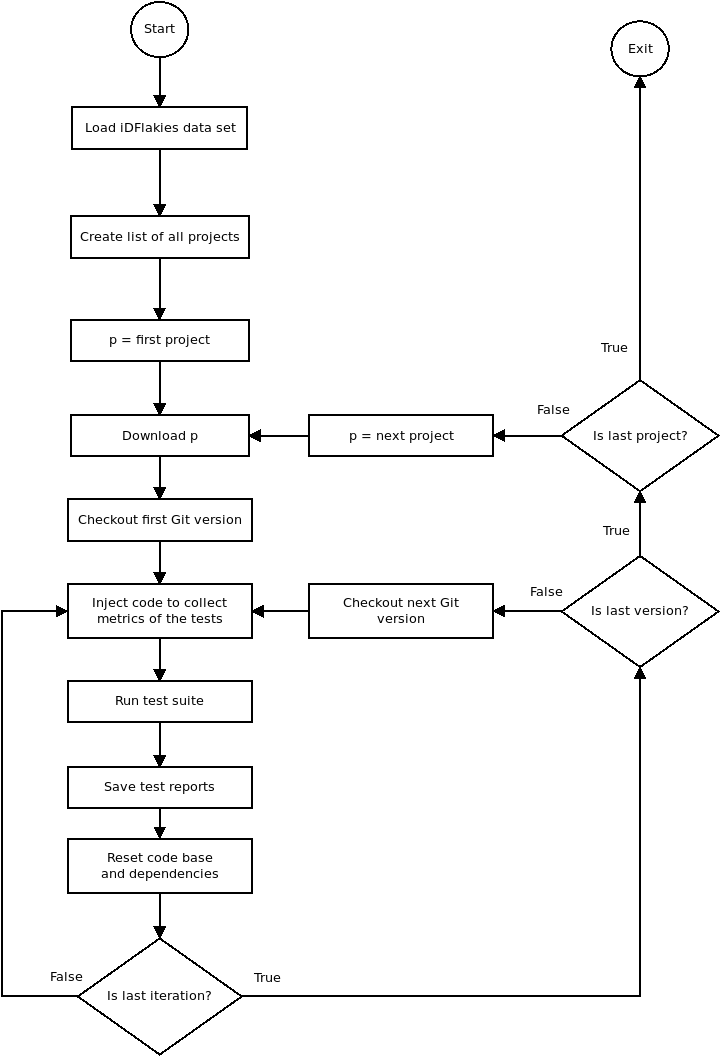
\includegraphics[scale=0.5]{images/toolchain_flow}
  \caption{High-level flow diagram of the toolchain.}
  \label{fig:toolchain}
\end{figure}

\subsection{Code injection} \label{sec:code_injection}
An important aspect of this toolchain is the process of injecting the code for taking the actual measurements of the JVM. A first approach was to use a Java agent, which allows to change the byte code of the classes during run-time. Java agents are interesting to change code because it is possible to take an already compiled project and instrument it without re-compiling from source. A Java agent can be attached to a JVM at start so that before the execution of the main method of the application a so called \textit{premain} method is called. This \textit{premain} method allows as mentioned above to add an instrumentation tool by using the provided Java \textit{Instrumentation} API. Java agents and the \textit{Instrumentation} API are not new features in the Java ecosystem since they are already specified in Java 5 \cite{java5}. The concrete bytecode manipulation could be done with \textit{ASM} developed by \textit{Bruneton et al.} \cite{bruneton02}, which is a Java library for manipulating Java class files. This library is low level and it requires more time to implement an agent than using the \textit{Bytebuddy} \cite{bytebuddy} library. \textit{Bytebuddy} depends only on the \textit{ASM} library. Therefore, \textit{Bytebuddy} can be viewed as an wrapper of \textit{ASM}, which also provides some interfaces that allow to develop in a consistent way. Although the approach with a Java agent to incect code to collect metrics of a test case seems to be good because there is no need to change the source code it has some difficulties in the environment of the toolchain. For developing a toolchain which runs several test suites of different Maven projects it is necessary to assume some convention that the projects follow. Since the projects are all Maven projects they must have a \textit{pom.xml} where the agent can be attached via the \textit{Surefire} plugin configuration. The problem is that most projects are multi module projects with multiple \textit{pom.xml} files and with multiple Maven profile configurations. So each \textit{pom.xml} of all projects need to be adjusted individually. However, this fact make it difficult to automate that very process. Therefore, an other approach to inject the code for taking the measurements was taken. \\

\noindent Since the approach with a Java agent has some problems in terms of attaching the agent at the JVM in an automated manner via the \textit{pom.xml} files an other solution should do this. Another assumption besides of having a \textit{pom.xml} file is the fact that Maven projects follow always a certain folder structure. The folder structure separates the application code from the test code. So it is possible to manipulate the test code on the source code level. The drawback is that it is not possible to attach the code manipulation dynamically during run-time like an Java agent. Furthermore, we have also to take into account that the projects need to be re-compiled, which also require time and therefore slow down the toolchain. The stage of injecting code into the source files of the tests is done in a separate Java process since the injection is implemented in Java with \textit{JavaParser} \cite{javaparser} whereas the toolcahin script is written in Python. \\

\noindent The toolchain invokes the source code injector by running its fat jar (jar with all dependencies included) with the appropriate arguments. The following listing \ref{injector} shows how to start the code injector.


\begin{lstlisting}[caption=Call source code injector,label=injector]
java -jar /path/to/jar /path/to/project projectName commitHash currentIteration
\end{lstlisting}

\noindent Besides the path to the source code injector fat jar there are also 4 more arguments. These arguments are needed to give additional information to the measurements which are also written to the \textit{csv} file. The following table \ref{tab:args} explains the arguments.



\begin{table}[ht]
\centering
\begin{tabular}{|l|l|}
\hline
\textbf{Argument} & \textbf{Explanation} \\ \hline
/path/to/jar & Path to the fat jar of the code injector \\ \hline
/path/to/project & Path to the target Maven project to instrument \\ \hline
  projectName & Name of target project (needed for \textit{csv} file) \\ \hline
commitHash & Version identifier of the target project \\ \hline
  currentIteration & Current run of the test suite \\ \hline
\end{tabular}
\caption{Explanation of the arguments for the code injector}
\label{tab:args}
\end{table}



\noindent The injected code uses a library from \textit{Dropwizard Metrics} \cite{dropwizard} to take measurements of the JVM. The tables \ref{tab:detailed-heap_metrics1} and \ref{tab:detailed-heap_metrics2} show an overview of all metrics that are memory related. The table \ref{tab:thread_metrics} summarizes the metrics of threads in the JVM. Furthermore, the table \ref{tab:garbage-collector_metrics} shows the metrics that are related to the JVM garbage collector.




\subsection{ScienceCloud} \label{sec:science_cloud}
The execution environments of the toolchain were \textit{ScienceCloud} instances of the University of Zurich \cite{cloud}. To run the toolchain on a local machine was not feasible since the run-time took about 70 hours. To overcome this issue the toolchain was run remotely. The first runs were done with a virtual machine that has 1GB of RAM and 1 virtual CPU. This configuration was chosen since it is the smallest that was available on \textit{ScienceCloud} to save computing resources. After looking the results and especially looking at the dump files it turned out that 1GB of RAM was not enough. Therefore two more runs are started with different configurations. One machine had 16 GB of RAM and 4 virtual CPU. The second one had 128 GB of RAM with 16 virtual CPUs. Later we call these machines machine A and machine B accordingly. All virtual machines had a Ubuntu 18.04 operating system running.


\section{Feature selection} \label{sec:cfs}
The post processed data set contains 72 variables in total. For doing further analysis on this data and especially to train classifiers  on this data we want to avoid overfitting.  overfitting occurs when too much data points is used for training. This leads to models, which do not generalize the data well. It is likely that couple of the variables are redundant and or irrelevant to do a binary classification whether test is flaky or not. Many machine learning algorithms  are costly in terms of  fitting the models. This is clearly true because with more features we also have more data, which needs to be processed of the computer. The field of machine learning algorithms and feature selection is broad and it is not the objective of this thesis. However, we need a method to overcome the problem of overfitting and feature irrelevance. \textit{Ghotra et al.} \cite{ghotra17} published a large-scale study on the impact of different feature selection techniques. Their objective was to identify a  selection technique that outperforms best among  the most known machine learning classifiers. They figured out that a correlation-based filter-subset technique with the \textit{BestFirst} search algorithm performs in general best. Therefore, for this thesis we used this method to do a feature selection. \\

\noindent The correlation based filter subset technique is composed of two parts. For the first part a heuristic function is required and for the second part a search algorithm is needed. With these two components we identify generally the best features for the most classifiers. \textit{Hall et al.} \cite{hall97} defined a heuristic function that is correlation based.  This function considers a whole group of features rather only single features.  The heuristic function  checks correlation of the features with the class label and the inter-correlation among the features. Therefore, it is  also called a filter-subset technique. The following equation \ref{eq:cfs} describes the heuristic function for a subset of features \cite{hall97}. \\


\begin{equation}
\label{eq:cfs}
G_s = \frac{k*\overline{r_{ci}}}{\sqrt{k + k * (k - 1) * \overline{r_{ii'}}}},
\end{equation}

\noindent where $k$ is the cardinality of the feature subset $G_s$, and $\overline{r_{ci}}$ is the average Pearson's correlation score between the class label and the features. The denominator considers the average Pearson's correlation score $\overline{r_{ii'}}$ among the features themselves. From this equation it s clear that correlation among the features should be low to get a higher heuristic score. \\

\noindent For the second part, \textit{Ghotra et al.} \cite{ghotra17} showed in their study got the correlation-based feature subset selection technique should be combined with the \textit{BestFirst} search algorithm. The best first search method is a graph algorithm.  The nodes of the graph represent a feature subset  which has a heuristic value.  The heuristic value is obtained from the formula above.  The aim of the best first search algorithm is to walk through the graph and search for the node that has the best heuristic value. 


\section{Classifiers} \label{sec:classifier}
In this thesis our aim is to do a binary classification  whether a certain test is flaky or not based on the runtime metrics we have collected. For this reason we evaluate 8 classifiers on their prediction performances. We have chosen four parametric classifiers and four non-parametric classifiers.  first we will take a look at the parametric classifiers and discuss their properties and how they work.  After this, we will discuss the non-parametric classifiers and outline their properties. \\

\subsection{Parametric}
\noindent The first parametric classifier we take a look at is the \textbf{Linear Discriminant Analysis} classifier or for short LDA. The LDA looks at the variances of the different groups (in our case only two) and define a classification line  separate the groups. In the one-dimensional case we can illustrate this separation by throwing the classification line where the  distributions of the groups intersect. This method can also be applied on more  than one variable. \\

\noindent In case where the variances of the groups  differ  then the LDA might be insufficient. The \textbf{Quadratic Discriminant Analysis} (QDA) classifier Could be a better solution. Instead of calculating the intersection of the densities the QDA takes the intersection of the log-densities. \\

\noindent The next method is the \textbf{Naive Bayes} classifier. This classifier uses the Bayes theorem that describes a probability of an event. This probability is based on a prior knowledge which effects the probability of  occurring  a certain event. \\

\noindent The last parametric classifier we look at is the \textbf{Logistic Regression}.  The purpose of the logistic regression is to model the probabilities occurring an event based on a set of features. The probabilities are linked with a link function to an ordinary linear regression model. The inverse of this link function is the logistic function. \\

\subsection{Non-parametric}
\noindent The first non-parametric classifier we look at is the \textbf{Classification Tree} classifier, which is also called as regression tree classifier. This classification method uses the approach of defining a set of rules to split the domain of a feature to classify  the observation to a group. At each successive step a feature is selected to discriminate between one group and the other. In the end we have a set of rules where to split the domains of the variables to obtain a classification model. \\

\noindent A more sophisticated approach, which also uses the idea of classification trees is the \textbf{Random Forest} classifier. The main idea behind this classifier is to grow multiple classification trees, which build a forest. The classification trees in the forest are not the same and can therefore lead to a different prediction. The random forest classifiers predict the outcome which has the most votes. \\

\noindent \textbf{Adaptive Boosting} (AdaBoost) belongs to the boosting algorithms that apply the same model multiple times but in each iteration the model is optimized based on the previous outcome. \\

\noindent \textbf{Extreme Gradient Boosting} (XGBoost) \cite{xgboost} is an optimized implementation of gradient boosting. Gradient boosting is in general used for classical regression and classification problems.




\section{Cross-validation}
For the evaluation of the different classifiers a special kind of cross-validation technique is used namely the \textit{stratified 10-fold cross-validation}. This approach differs from the classic k-fold cross-validation in the folding of the data. In our case we have \textit{a priori} knowledge of having an imbalanced data set where the number of flaky tests is much lower than the non-flaky tests. This assumption verifies also \textit{Micco} \cite{micco17} who showed that Google has 1.5\% flaky tests in their test suites. So flaky tests are rare events and must be treated carefully. The \textit{stratified 10-fold cross-validation} is a way to tackle the problem of imbalanced data in machine learning. This type of cross-validation ensures that the distribution of the class labels are as similar as possible over the different folds \cite{qian09}. It is important that there is no fold with only one class label. If there is only one class represented in a fold then the performance scores will calculate no reliable values.

\section{Threats to validity}
The methodology above has also some threats to validity. The whole thesis is limited to projects in the Java ecosystem. In particular all the projects are open-source projects that use the Maven build tool. The according pom files of the projects follow not always the same structure which can affect the source code injector. Furthermore, the used projects are from the \textit{iDFlakies} data set. There is no other large public data set on known flaky tests. This data set is limited to only 82 projects. For the classification models the default parameters of the \textit{sklearn} library is used. The defaults are usually not the best and with parameter optimization a significant better prediction performance is possible. Some projects may have very specific requirements to run the tests but in order to automate the test execution of 82 projects it is likely that some specific requirements were not met. For all projects the same JDK vendor was used and the same Java 8 version. The test execution was also done in a virtual machine on \textit{ScienceCloud}. A virtual machine on a server may impact the execution of the toolchain and lead to a different result than the execution of the toolchain on a personal computer. 




\chapter{Results}
In the following sections you will find the main results of the data analysis. To get a first impression of the data and to see how the structure of the data of flaky tests are  we did a PCA and a biplot to reduce the dimensionality. The second part you examines the tables that summarize the cross-validation results of different classifiers. Those tables shall answer the research questions.
\section{PCA}
To identify a cluster structure among multivariate data a PCA with an according biplot of the \textit{hadoop} project on machine A was done. The \textit{hadoop} project has the most identified flaky tests. In figure \ref{fig:biplot} you see the biplot  of the data of the \textit{hadoop} project on machine A. By a dimension reduction a cluster structure is identified but not completely separated from the non-flaky data points. \\ 

\begin{figure}[ht]
  \centering
  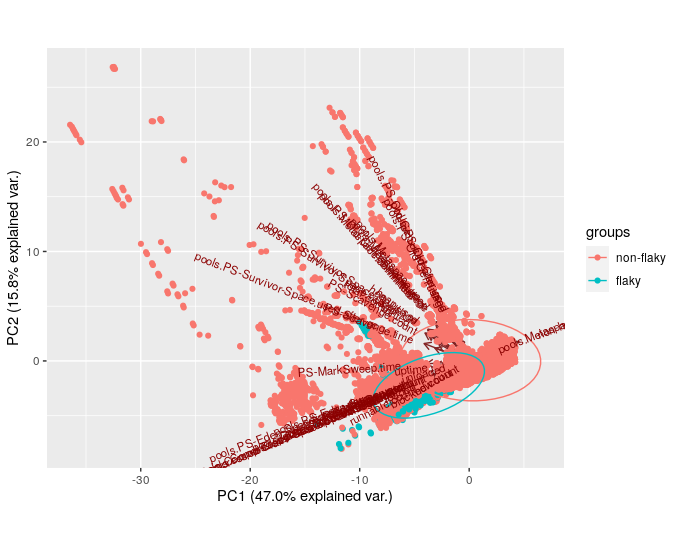
\includegraphics[scale=0.6]{images/hadoop-vm9-own}
  \caption{PCA biplot of hadoop's flaky tests}
  \label{fig:biplot}
\end{figure}

\noindent Other software projects have less identified flaky tests than the \textit{hadoop} project. Biplots for the other projects would not give a valuable insight since the data for those projects are too imbalanced.

\section{Cross-validation}
The following sections show the results of various stratified 10-fold cross-validations. Furthermore, the sections are organized so that for each machine the cross-validation is done based on the JVM metrics and on the metrics differences. The differences are taken to do the validation on data that are only test case related and not on the general state of the JVM. \\

\noindent The following abbreviations for the classifiers and its explanations will help to read the tables:
\begin{itemize}
\item lda: Linear Discriminant Analysis
\item qda: Quadratic Discriminant Analysis
\item gnbayes: Gaussian Naive Bayes
\item logreg: Logistic Regression
\item ctree: Classification Tree
\item rforest: Random Forest
\item adaboost: Ada Boosting
\item xgboost: Extreme Gradient Boosting
\end{itemize}

Here is also a list of the abbreviations for the cross-validation scores and its explanations:
\begin{itemize}
\item ACC: Accuracy
\item PREC: Precision
\item RECA: Recall
\item F1: F1 score
\item MCC: Mathew's Correlation Coefficient
\item AUC: Area under the ROC curve
\end{itemize}



\subsection{Machine A}
In this section you will find the results of machine A which had the following specifications:

\begin{itemize}
\item Ubuntu 18.04
\item 4 vCPUs
\item 16 GB of RAM
\end{itemize}

\noindent Table \ref{tab:cvmachineAown} shows the results of the predicting performances of flaky tests that are identified by ourselves as flaky. Whereas table \ref{tab:cvmachineAidflakies} shows the results when using the labels from the iDflakies data set. The tables \ref{tab:cvmachineAownDiff} and \ref{tab:cvmachineAidflakiesDiff} uses the differences of before and after a test execution.\\

\noindent The results of the cross-validation for the data with own identified flaky tests in table \ref{tab:cvmachineAown} show that the gnbayes classifier perform worst if we consider the PREC, RECA, F1 and the MCC. The rforest classifier has the best AUC, MCC, F1 and RECA score. The simple classification tree performs almost identical to the random forest classifier. Although the non-parametric classifiers perform generally better than the parametric it is obvious that the adaboost classifier has poor PREC, RECA, F1, MCC and AUC scores.\\

\begin{table}[ht]
\centering
\begin{tabular}{|l|l|l|l|l|l|l|}
\hline
\textbf{Classifier} & \textbf{ACC} & \textbf{PREC} & \textbf{RECA} & \textbf{F1} & \textbf{MCC} & \textbf{AUC} \\ \hline
  lda & 0.9872 & 0.0664 & 0.4 & 0.1139 & 0.1591 & 0.6942 \\ \hline
  qda & 0.9844 & 0.0477 & 0.35 & 0.0839 & 0.1247 & 0.6678 \\ \hline
  gnbayes & 0.9968 & 0.0 & 0.0 & 0.0 & -0.0015 & 0.4994 \\ \hline
  logreg & 0.9979 & 0.15 & 0.0008 & 0.0017 & 0.0064 & 0.5004 \\ \hline
  ctree & 0.9987 & 0.7847 & 0.5149 & 0.6211 & 0.6347 & 0.7573 \\ \hline
  rforest & 0.9987 & 0.7745 & 0.5280 & 0.6275 & 0.6387 & 0.7638 \\ \hline
  adaboost & 0.9977 & 0.0126 & 0.0017 & 0.0030 & 0.0040 & 0.5007 \\ \hline
  xgboost & 0.9981 & 0.9442 & 0.1175 & 0.2076 & 0.3299 & 0.5587 \\ \hline
\end{tabular}
\caption{Stratified 10-fold cross-validation of own identified flaky tests for machine A.}
\label{tab:cvmachineAown}
\end{table}

\noindent If we take a look at the results of the cross-validation based on the metrics' differences then the logreg classifier has the poorest performance according to the RECA, F1, MCC and the AUC scores. The qda has a very low accuracy of 19.39\% although the data is highly imbalanced. The gnbayes classifier has in contrast to the previous table the larges AUC score but the accuracy is with 89.14\% low in comparison to the other classifiers and especially in contrast to the imbalanced data. The ctree and the rforest classifiers hava the highest PREC, F1 and MCC scores. \\

\begin{table}[ht]
\centering
\begin{tabular}{|l|l|l|l|l|l|l|}
\hline
\textbf{Classifier} & \textbf{ACC} & \textbf{PREC} & \textbf{RECA} & \textbf{F1} & \textbf{MCC} & \textbf{AUC} \\ \hline
  lda & 0.9942 & 0.2054 & 0.5053 & 0.2913 & 0.3193 & 0.7503 \\ \hline
  qda & 0.1939 & 0.0029 & 0.9875 & 0.0057 & 0.0222 & 0.5898 \\ \hline
  gnbayes & 0.8914 & 0.0174 & 0.8214 & 0.0340 & 0.1098 & 0.8565 \\ \hline
  logreg & 0.9976 & 0.8 & 0.0 & 0.0 & -6.2402e-05 & 0.4999 \\ \hline
  ctree & 0.9976 & 0.5155 & 0.2196 & 0.3067 & 0.3346 & 0.6095 \\ \hline
  rforest & 0.9976 & 0.5198 & 0.2232 & 0.3094 & 0.3377 & 0.6113 \\ \hline
  adaboost & 0.9974 & 0.1149 & 0.0553 & 0.0682 & 0.0741 & 0.5274 \\ \hline
  xgboost & 0.9976 & 0.5133 & 0.05 & 0.0767 & 0.1216 & 0.5249 \\ \hline
\end{tabular}
\caption{Stratified 10-fold cross-validation of own identified flaky tests for machine A with metrics differences.}
\label{tab:cvmachineAownDiff}
\end{table}


\noindent The scores of the cross-validations based on iDFlakies class labes and the absolute JVM metrics are shown in table \ref{tab:cvmachineAidflakies}. The table shows clearly that the parametric classifiers perform worst according the the PREC, RECA, F1, MCC and AUC. The rforest has the highest overall scores (except the PREC score) followed by the ctree classifier. Note that the xgboost has the highest PREC score but in general it performs worse than the rforest and the ctree classifier. In comparison to the results of the table \ref{tab:cvmachineAown} the rforest and the ctree classifiers have similar scores. The scores of the data with the class labels from iDFlakies are not significantly lower. \\


\begin{table}[ht]
\centering
\begin{tabular}{|l|l|l|l|l|l|l|}
\hline
\textbf{Classifier} & \textbf{ACC} & \textbf{PREC} & \textbf{RECA} & \textbf{F1} & \textbf{MCC} & \textbf{AUC} \\ \hline
lda & 0.9891 & 0.0 & 0.0 & 0.0 & -0.0024 & 0.4996 \\ \hline
qda & 0.9818 & 0.0177 & 0.0131 & 0.0149 & 0.0061 & 0.5025 \\ \hline
gnbayes & 0.9897 & 1.0 & 0.0 & 0.0 & 0.0 & 0.5 \\ \hline
logreg & 0.9897 & 0.1 & 0.0 & 0.0 & -0.0006 & 0.4999 \\ \hline
ctree & 0.9932 & 0.7795 & 0.4702 & 0.5865 & 0.6023 & 0.7344 \\ \hline
rforest & 0.9931 & 0.7701 & 0.4763 & 0.5885 & 0.6026 & 0.7374 \\ \hline
adaboost & 0.9899 & 0.7523 & 0.0195 & 0.0378 & 0.1098 & 0.5097 \\ \hline
xgboost & 0.9908 & 0.9300 & 0.1195 & 0.2117 & 0.3315 & 0.5597 \\ \hline
\end{tabular}
\caption{Stratified 10-fold cross-validation of flaky tests identified by iDFlakies for machine A.}
\label{tab:cvmachineAidflakies}
\end{table}



\noindent The table \ref{tab:cvmachineAidflakiesDiff} shows the results of the data with the metrics' differences and the class labels from iDFlakies. We see that the rforest and the ctree classifiers have the highest MCC scores but in comparison to the previous results they are low. Overall, all the scores for all classifiers are low. Like the previous results also here are the rforest and the ctree classifiers similar in their performances.

\begin{table}[ht]
\centering
\begin{tabular}{|l|l|l|l|l|l|l|}
\hline
\textbf{Classifier} & \textbf{ACC} & \textbf{PREC} & \textbf{RECA} & \textbf{F1} & \textbf{MCC} & \textbf{AUC} \\ \hline
  lda & 0.9882 & 0.0769 & 0.0172 & 0.0281 & 0.0318 & 0.5075 \\ \hline
  qda & 0.9561 & 0.0563 & 0.2189 & 0.0896 & 0.0938 & 0.5912 \\ \hline
  gnbayes & 0.9596 & 0.0526 & 0.1818 & 0.0816 & 0.0813 & 0.5746 \\ \hline
  logreg & 0.9901 & 0.7083 & 0.0084 & 0.0166 & 0.0747 & 0.5041 \\ \hline
  ctree & 0.9902 & 0.5917 & 0.0523 & 0.0956 & 0.1722 & 0.5259 \\ \hline
  rforest & 0.9902 & 0.5990 & 0.0535 & 0.0978 & 0.1755 & 0.5266 \\ \hline
  adaboost & 0.9901 & 0.6916 & 0.0042 & 0.0083 & 0.0435 & 0.5020 \\ \hline
  xgboost & 0.9903 & 0.8248 & 0.0282 & 0.0544 & 0.1496 & 0.5141 \\ \hline
\end{tabular}
\caption{Stratified 10-fold cross-validation of flaky tests identified by iDFlakies for machine A with metrics differences.}
\label{tab:cvmachineAidflakiesDiff}
\end{table}


\subsection{Machine B}
In this section you will find the results of machine B which had the following specifications:

\begin{itemize}
\item Ubuntu 18.04
\item 16 vCPUs
\item 128 GB of RAM
\end{itemize}

\noindent Like for machine A the results are organized in the same way. Tables \ref{tab:cvmachineBown} and \ref{tab:cvmachineBidflakies} uses different sources for the labels and consider the general state of the JVM. Tables \ref{tab:cvmachineBownDiff} and \ref{tab:cvmachineBidflakiesDiff} show the results performed on the data based on the differences (after test execution minus before test execution). \\

\noindent The table \ref{tab:cvmachineBown} shows the results of the cross-validations with the absolute JVM metrics data and the own identified flaky tests as the positive class labels. We see that the logreg classifier has the worst scores especially the PREC, RECA and F1 are equal to zero. Furthermore, the MCC and the AUC scores are the lowest in comparison to the other classifiers. The rforest and the ctree classifiers have for all scores a value over 90\% (except for RECA of ctree with 89.44\%). The xgboost classifier has similar scores like rforest and ctree but the RECA, F1 and MCC are between 85\% and 90\%. The adaboost classifier has for the previous mentioned scores lower values than xgboost classifier. The values ranges between 78\% and 82\%. Note that the parametric classifier perform worst according to the F1, MCC and PREC scores. \\



\begin{table}[ht]
\centering
\begin{tabular}{|l|l|l|l|l|l|l|}
\hline
\textbf{Classifier} & \textbf{ACC} & \textbf{PREC} & \textbf{RECA} & \textbf{F1} & \textbf{MCC} & \textbf{AUC} \\ \hline
lda & 0.9911 & 0.1603 & 0.9045 & 0.2723 & 0.3787 & 0.9479 \\ \hline
qda & 0.9886 & 0.1306 & 0.9201 & 0.2287 & 0.3443 & 0.9544 \\ \hline
gnbayes & 0.9766 & 0.0680 & 0.9256 & 0.1268 & 0.2476 & 0.9512 \\ \hline
logreg & 0.9979 & 0.0 & 0.0 & 0.0 & -0.0005 & 0.4999 \\ \hline
ctree & 0.9996 & 0.9306 & 0.8944 & 0.9119 & 0.9120 & 0.9471 \\ \hline
rforest & 0.9997 & 0.9355 & 0.9009 & 0.9176 & 0.9177 & 0.9504 \\ \hline
adaboost & 0.9993 & 0.8556 & 0.7871 & 0.8192 & 0.8199 & 0.8934 \\ \hline
xgboost & 0.9995 & 0.9174 & 0.8559 & 0.8855 & 0.8859 & 0.9279 \\ \hline
\end{tabular}
\caption{Stratified 10-fold cross-validation of own identfied flaky tests for machine B.}
\label{tab:cvmachineBown}
\end{table}


\noindent The table \ref{tab:cvmachineBownDiff} shows the cross-validation results based on the JVM metrics' differences and with the positive class labels for own identified flaky tests. From the table it is obvious to see that all classifiers have poor scores in comparison to all previous results. To note is that here the rforest and the ctree classifiers have similar scores. Furthermore, these two classifiers are the best in the table although their scores are in comparison to other tables low. \\



\begin{table}[ht]
\centering
\begin{tabular}{|l|l|l|l|l|l|l|}
\hline
\textbf{Classifier} & \textbf{ACC} & \textbf{PREC} & \textbf{RECA} & \textbf{F1} & \textbf{MCC} & \textbf{AUC} \\ \hline
  lda & 0.9970 & 0.0 & 0.0 & 0.0 & -0.0007 & 0.4986 \\ \hline
  qda & 0.0002 & 0.0002 & 1.0 & 0.0004 & 0.0 & 0.5 \\ \hline
  gnbayes & 0.9950 & 0.1 & 0.0 & 0.0 & -0.0010 & 0.4976 \\ \hline
  logreg & 0.9997 & 1.0 & 0.0 & 0.0 & 0.0 & 0.5 \\ \hline
  ctree & 0.9997 & 0.3833 & 0.05 & 0.0757 & 0.0931 & 0.5249 \\ \hline
  rforest & 0.9997 & 0.3833 & 0.0333 & 0.0472 & 0.0523 & 0.5166 \\ \hline
  adaboost & 0.9997 & 0.9 & 0.0 & 0.0 & -9.5786e-06 & 0.4999 \\ \hline
  xgboost & 0.9997 & 1.0 & 0.0 & 0.0 & 0.0 & 0.5 \\ \hline
\end{tabular}
\caption{Stratified 10-fold cross-validation of own identfied flaky tests for machine B with metrics differences.}
\label{tab:cvmachineBownDiff}
\end{table}



\noindent The following table \ref{tab:cvmachineBidflakies} shows the cross-validation results based on the absolute JVM metrics and with the positive class labels from the iDFlakies data set. The logreg classifier has the worst RECA, F1, MCC and AUC scores. The scores for the parametric classifiers all below 20\% for RECA, F1 and MCC. The non-parametric classifier perform similar or better than the parametric classifiers. The rforest and the ctree classifiers have the highest RECA, F1, MCC and AUC scores. The xgboost classifier perform best according to the PREC but the scores for RECA, F1 and MCC are lower than 36\%. The adaboost perform for all scores worse than xgboost. \\



\begin{table}[ht]
\centering
\begin{tabular}{|l|l|l|l|l|l|l|}
\hline
\textbf{Classifier} & \textbf{ACC} & \textbf{PREC} & \textbf{RECA} & \textbf{F1} & \textbf{MCC} & \textbf{AUC} \\ \hline
  lda & 0.9834 & 0.1419 & 0.1074 & 0.1222 & 0.1152 & 0.5502 \\ \hline
  qda & 0.9782 & 0.1167 & 0.1566 & 0.1337 & 0.1243 & 0.5719 \\ \hline
  gnbayes & 0.9641 & 0.0599 & 0.1595 & 0.0871 & 0.0818 & 0.5661 \\ \hline
  logreg & 0.9892 & 1.0 & 0.0 & 0.0 & 0.0 & 0.5 \\ \hline
  ctree & 0.9928 & 0.7012 & 0.5890 & 0.6401 & 0.6391 & 0.7931 \\ \hline
  rforest & 0.9931 & 0.7225 & 0.5835 & 0.6455 & 0.6458 & 0.7905 \\ \hline
  adaboost & 0.9901 & 0.8943 & 0.0933 & 0.1686 & 0.2862 & 0.5466 \\ \hline
  xgboost & 0.9906 & 0.9185 & 0.1427 & 0.2469 & 0.3598 & 0.5713 \\ \hline
\end{tabular}
\caption{Stratified 10-fold cross-validation of flaky tests identified by iDFlakies for machine B.}
\label{tab:cvmachineBidflakies}
\end{table}



\noindent The table \ref{tab:cvmachineBidflakiesDiff} shows the cross-validation results based on the differences of the JVM metrics with the positive class labels from the iDFlakies data set. In this table we see again as from the previous results that the rforest and the ctree classifiers perform best. In particular they have the best RECA, F1, MCC and AUC scores. The results show that the parametric classifiers have for the RECA, F1 and MCC scores no value over 25\%. The xgboost classifier has for all scores low values and the adaboost classifier is also here even worse than the xgboost classifier. These results also show that the rforest and the ctree classifier have similar scores but the rforest is overall slightly better by 1\%. \\


\begin{table}[ht]
\centering
\begin{tabular}{|l|l|l|l|l|l|l|}
\hline
\textbf{Classifier} & \textbf{ACC} & \textbf{PREC} & \textbf{RECA} & \textbf{F1} & \textbf{MCC} & \textbf{AUC} \\ \hline
  lda & 0.9827 & 0.0618 & 0.0452 & 0.0522 & 0.0443 & 0.5189 \\ \hline
  qda & 0.9516 & 0.0595 & 0.2425 & 0.0956 & 0.1016 & 0.6008 \\ \hline
  gnbayes & 0.9525 & 0.0558 & 0.2203 & 0.0891 & 0.0924 & 0.5903 \\ \hline
  logreg & 0.9895 & 0.6797 & 0.0081 & 0.0160 & 0.0699 & 0.5040 \\ \hline
  ctree & 0.9907 & 0.6077 & 0.3582 & 0.4500 & 0.4619 & 0.6779 \\ \hline
  rforest & 0.9910 & 0.6284 & 0.3653 & 0.4615 & 0.4747 & 0.6815 \\ \hline
  adaboost & 0.9892 & 0.1342 & 0.0007 & 0.0014 & 0.0037 & 0.5002 \\ \hline
  xgboost & 0.9898 & 0.9002 & 0.0370 & 0.0708 & 0.1784 & 0.5185 \\ \hline
\end{tabular}
\caption{Stratified 10-fold cross-validation of flaky tests identified by iDFlakies for machine B with metrics differences.}
\label{tab:cvmachineBidflakiesDiff}
\end{table}

\noindent For both execution environments machine A and B the rforest and the ctree classifiers perform in general best followed by the xgboost classifier. In particular we also see that the scores are better if we use the absolute JVM metrics and not the differences. This observation is made by machine A and B. If we compare the impact of the different memory size of machine A and B then we also see that machine B with 128GB of RAM have in general better scores than the cross-validation results of machine A with 16 GB of RAM. 


\chapter{Discussion}
Since flaky tests are a big issue in the industry it is important to investigate different mitigation strategies. Our findings show that there are certain cluster structures of flaky tests based on JVM metrics. Such clusters can enhance the predictability of different machine learning models. Indeed, this thesis has shown that flaky tests can be predicted by machine learning models. This approach is quite different in comparison with the current methods for dealing with flaky tests like \textit{Rerun} and \textit{DeFlaker}. It requires more research to optimize a machine learning based on JVM metrics. Furthermore, a deep learning approach could perform differently but it was not a part of this thesis. In general, such classifiers can be integrated in a custom Java test runner to indicate also a passing test as possibly flaky. With such a test runner there would be no need to have only failing tests to do a rerun since we know based on the JVM metrics that also a passing test can be flaky on later runs. In the context of having a continuous integration pipeline such a test runner can improve the developers' efficiency. If the test runner shows that a certain test case is likely to be flaky and the test fails then the developer can rather try to fix the flakiness instead of fixing a nonexistent defect in the code under test. Such a tool will probably have a larger impact on big software projects so that no unnecessary costs of fixing nonexistent defects can be minimized. \\

\noindent The results of this thesis give no essential information why flakiness occurs or what additional root causes of flakiness are which are already discussed in previous related work. But the results supports the results and findings from the Google blog post by \textit{Listfield} \cite{listfield17}, that shows a relationship between memory consumption and the probability of flakiness of a test. Furthermore, this thesis uses data with different metrics of different JVM memory areas. This gives a more detailed and specialized results. An important observation is that the general predictability of flaky tests is better with data that uses metrics of the whole JVM as absolute values. Data that uses the difference between the metrics of after a test execution and the metrics before a test execution lead to a poorer predictability. With the differences a test only related data set is used which neglect the absolute values of the JVM. \\

\noindent The findings of this thesis shows that flaky tests can be predicted based on JVM metrics. Future research shall also focus on native applications that are not developed in the Java ecosystem. Furthermore, it would be interesting how flaky tests behave in scripting languages like Python and Javascript. Can flaky tests in those languages also be predicted by machine learning models and memory related data? Since there are also root causes that are network related an extension of the data with network related metrics can be interesting. For example besides having a data set with memory related metrics two additional variables that give some measures about the upload and download sizes of the current test execution. This thesis has also shown that there is a difference between the predictability of flaky tests of machine A and machine B that have different memory sizes. It is worth to investigate more the impact of memory sizes on the flakiness of tests. This thesis used only two different machines that give not yet a reliable answer if larger memory really minimizes the flakiness of tests. Another aspect which was not investigated so far is the impact of parameter optimization of the classifier on the predictability. In this thesis we used the default parameters for the different classifiers. In machine learning it is usually the case that some improvement can be done by optimizing the parameters of the models. \\

\noindent Another interesting approach for further research would be to investigate the impact of bytecode frequency of flaky tests. Likewise for native applications outside of the Java ecosystem the opcodes frequencies can be used for flaky test classification. This would be a similar approach as how some malware detection software work. If the development of better dynamic strategies for dealing flaky tests progress then the costs of rerun the failing tests in test suite can be lowered. On a large scale project this could have a significant impact by minimizing the useless reruns. As software project become more complex in the future software developer shall give more attention to the impact of flaky tests. This thesis gives a motivation to do further research in predicting flaky tests and to develop more mitigation strategies with its insights.






\chapter{Conclusion}
In this thesis we investigated the impact of JVM metrics on the predictability of flaky tests. Furthermore, we were interested in if there is a cluster structure in the JVM metrics among flaky tests. The data set of the \textit{iDFlakies} project gives the basis information of flaky tests on 82 open-source projects. In order to collect JVM metrics we developed a toolchain that executed the test suites of the projects with a modified code base so that JVM metrics are collected. \\

\noindent To understand the structure of flaky tests in the data a PCA with a biplot was done. Since there are too many data for giving a plot we needed the project with the most identified flaky tests. The \textit{hadoop} had the most flaky tests and the biplot indicates clearly that the flaky tests are grouped together in a dimension reduced space based on the first and second principle components on absolute JVM metrics. \\

\noindent The following paragraphs will answer the research questions:

\paragraph{RQ1} First the non-parametric models perform in general better than the parametric ones. Especially the random forest and the classification tree models performed best. The extreme gradient boosting model performs third best.

\paragraph{RQ2} Furthermore, the predictability is better by using absolute JVM metrics than only the differences used by a single test.

\paragraph{RQ3} An interesting observation is also that different sizes of RAM also impact the predictability. Data of machine B with 128 GB of RAM generally performed better. 

\paragraph{RQ4} The performance of prediction is lower if we used the flaky labels from the \textit{iDFlakies} data set. To use class labels from different data sources will lead to the problem that the execution environment is likely not identical. As mentioned above we see that the RAM size has also an impact. \\

\noindent The insights of this thesis allows to predict flaky tests at a certain degree. The prediction allows to know if a test is flaky although the test passes. It is not necessary anymore to have failing test beforehand in order to identify flaky tests. This thesis should enable future research on predicting flaky tests by machine learning models. There are still many things which are not considered so far (e.g., network usage, flaky tests of non-Java projects, scripting languages, etc.). These new insights can give more motivation in developing new tools for mitigating flaky tests. Such tool have the potential to increase the productivity during development and to lower the costs.

\backmatter
\bibliographystyle{ieeetr}
\bibliography{literature}

\chapter{Appendix}


% table for metrics
\begin{table}[ht]
\centering
\begin{tabular}{|l|l|}
\hline
\textbf{Metric} & \textbf{Explanation} \\ \hline
heap.committed	& The amount of memory in bytes that is \\ 
				& committed for the Java virtual machine to use \\ \hline
heap.init 		& The amount of memory in bytes that the \\
				& Java virtual machine initially requests \\
				& from the operating system for \\
				& memory management \\ \hline
heap.max 		& The maximum amount of memory in bytes that \\
				& can be used for memory management \\ \hline
heap.usage & Ratio used / max \\ \hline
heap.used & The amount of used memory in bytes \\ \hline
non-heap.committed & The amount of memory in bytes that is \\
				& committed for the Java virtual machine to use \\ \hline
non-heap.init 	& The amount of memory in bytes that the Java \\
				& virtual machine initially requests from the \\
				& operating system for memory management \\ \hline
non-heap.max 	& The maximum amount of memory in bytes that \\
				& can be used for memory management \\ \hline
non-heap.usage 	& Ratio used / max \\ \hline
non-heap.used 	& The amount of used memory in bytes \\ \hline
pools.Code-Cache.committed 	& The amount of memory in bytes that \\
							& is committed for the Java virtual machine to use \\ \hline
pools.Code-Cache.init & The amount of memory in bytes that the Java \\
						& virtual machine initially requests from the \\
						& operating system for memory management \\ \hline
pools.Code-Cache.max 	& The maximum amount of memory in bytes that \\
						& can be used for memory management \\ \hline
pools.Code-Cache.usage & Ratio used / max \\ \hline
pools.Code-Cache.used & The amount of used memory in bytes \\ \hline
pools.Compressed-Class-Space.committed & The amount of memory in bytes that is \\
					& committed for the Java virtual machine to use \\ \hline
pools.Compressed-Class-Space.init & The amount of memory in bytes that the Java \\ 
									& virtual machine initially requests from the \\
									& operating system for memory management \\ \hline
pools.Compressed-Class-Space.max & The maximum amount of memory in bytes that \\
								&  can be used for memory management \\ \hline
pools.Compressed-Class-Space.usage & Ratio used / max \\ \hline
pools.Compressed-Class-Space.used & The amount of used memory in bytes \\ \hline
pools.Metaspace.committed & The amount of memory in bytes that \\
							& is committed for the Java virtual machine to use \\ \hline
pools.Metaspace.init & The amount of memory in bytes that the Java \\
					& virtual machine initially requests from the \\
					& operating system for memory management \\ \hline
pools.Metaspace.max & The maximum amount of memory in bytes that \\
					& can be used for memory management \\ \hline
pools.Metaspace.usage & Ratio used / max \\ \hline
pools.Metaspace.used & The amount of used memory in bytes \\ \hline

\end{tabular}
\caption{Explanation of detailed memory metrics part 1}
\label{tab:detailed-heap_metrics1}
\end{table}


\begin{table}[ht]
\centering
\begin{tabular}{|l|l|}
\hline
\textbf{Metric} & \textbf{Explanation} \\ \hline
pools.PS-Eden-Space.committed & The amount of memory in bytes that is \\
								& committed for the Java virtual machine to use \\ \hline
pools.PS-Eden-Space.init & The amount of memory in bytes that \\
							& the Java virtual machine initially requests from the \\
							& operating system for memory management \\ \hline
pools.PS-Eden-Space.max & The maximum amount of memory in bytes that \\
						& can be used for memory management \\ \hline
pools.PS-Eden-Space.usage & Ratio used / max \\ \hline
pools.PS-Eden-Space.used & The amount of used memory in bytes \\ \hline
pools.PS-Eden-Space.used-after-gc & \\ \hline
pools.PS-Old-Gen.committed & The amount of memory in bytes that is \\
							& committed for the Java virtual machine to use \\ \hline
pools.PS-Old-Gen.init & The amount of memory in bytes that \\
						& the Java virtual machine initially requests from the \\
						& operating system for memory management \\ \hline
pools.PS-Old-Gen.max & The maximum amount of memory in bytes that \\
						& can be used for memory management \\ \hline
pools.PS-Old-Gen.usage & Ratio used / max \\ \hline
pools.PS-Old-Gen.used & The amount of used memory in bytes \\ \hline
pools.PS-Old-Gen.used-after-gc & \\ \hline
pools.PS-Survivor-Space.committed & The amount of memory in bytes that is \\
									& committed for the Java virtual machine to use \\ \hline
pools.PS-Survivor-Space.init & The amount of memory in bytes that \\
							& the Java virtual machine initially requests from the \\
							& operating system for memory management \\ \hline
pools.PS-Survivor-Space.max & The maximum amount of memory in bytes that \\
							& can be used for memory management \\ \hline
pools.PS-Survivor-Space.usage & Ratio used / max \\ \hline
pools.PS-Survivor-Space.used & The amount of used memory in bytes \\ \hline
pools.PS-Survivor-Space.used-after-gc & \\ \hline
total.committed & The amount of memory in bytes that is \\
									& committed for the Java virtual machine to use \\ \hline
total.init & The amount of memory in bytes that \\
							& the Java virtual machine initially requests from the \\
							& operating system for memory management \\ \hline
total.max & The maximum amount of memory in bytes that \\
							& can be used for memory management \\ \hline
total.used & The amount of used memory in bytes \\ \hline
\end{tabular}
\caption{Explanation of detailed memory metrics part 2}
\label{tab:detailed-heap_metrics2}
\end{table}






% table for metrics
\begin{table}[ht]
\centering
\begin{tabular}{|l|l|}
\hline
\textbf{Metric} & \textbf{Explanation} \\ \hline
PS-MarkSweep.count & The total number of collections that have occurred\\ \hline
PS-MarkSweep.time & The approximate accumulated collection elapsed time in milliseconds\\ \hline
PS-Scavenge.count & The total number of collections that have occurred \\ \hline
PS-Scavenge.time & The approximate accumulated collection elapsed time in milliseconds\\ \hline
\end{tabular}
\caption{Explanation of garbage collector metrics}
\label{tab:garbage-collector_metrics}
\end{table}


% table for metrics
\begin{table}[ht]
\centering
\begin{tabular}{|l|l|}
\hline
\textbf{Metric} & \textbf{Explanation} \\ \hline
blocked.count & Current number of threads in "blocked" state in this JVM \\ \hline
count & Current number of threads in this JVM\\ \hline
daemon.count & Current number of live daemon threads in this JVM \\ \hline
deadlock.count & Current number of deadlocked threads in this JVM \\ \hline
deadlocks & Collection of information about the currently deadlocked threads \\ \hline
new.count & Current number of threads in "new" state\\ \hline
runnable.count & Current number of threads in "runnable" state in this JVM \\ \hline
terminated.count & Current number of threads in "terminated" state \\ \hline
timed\_waiting.count & Current number of threads in "timed\_waiting" state in this JVM \\ \hline
waiting.count & Current number of threads in "waiting" state in this JVM \\ \hline
\end{tabular}
\caption{Explanation of thread metrics}
\label{tab:thread_metrics}
\end{table}


%%%%%%%%%%%%%%%%%%%%%%%%%%%%%%%%%
%%%%%%%%%%%%%%%%%%%%%%%%%%%%%%%%%


%
%% table for metrics
%\begin{table}[ht]
%\centering
%\begin{tabular}{|l|l|}
%\hline
%\textbf{Metric} & \textbf{Explanation} \\ \hline
%TestCase & \\ \hline
%ProjectName & \\ \hline
%CommitHash & \\ \hline
%pass/fail & \\ \hline
%before/after & \\ \hline
%PS-MarkSweep.count & \\ \hline
%PS-MarkSweep.time & \\ \hline
%PS-Scavenge.count & \\ \hline
%PS-Scavenge.time & \\ \hline
%blocked.count & \\ \hline
%count & \\ \hline
%daemon.count & \\ \hline
%deadlock.count & \\ \hline
%deadlocks & \\ \hline
%heap.committed & \\ \hline
%heap.init & \\ \hline
%heap.max & \\ \hline
%heap.usage & \\ \hline
%heap.used & \\ \hline
%loaded & \\ \hline
%name & \\ \hline
%new.count & \\ \hline
%non-heap.committed & \\ \hline
%non-heap.init & \\ \hline
%non-heap.max & \\ \hline
%non-heap.usage & \\ \hline
%non-heap.used & \\ \hline
%pools.Code-Cache.committed & \\ \hline
%pools.Code-Cache.init & \\ \hline
%pools.Code-Cache.max & \\ \hline
%pools.Code-Cache.usage & \\ \hline
%pools.Code-Cache.used & \\ \hline
%pools.Compressed-Class-Space.committed & \\ \hline
%pools.Compressed-Class-Space.init & \\ \hline
%pools.Compressed-Class-Space.max & \\ \hline
%pools.Compressed-Class-Space.usage & \\ \hline
%pools.Compressed-Class-Space.used & \\ \hline
%pools.Metaspace.committed & \\ \hline
%pools.Metaspace.init & \\ \hline
%pools.Metaspace.max & \\ \hline
%pools.Metaspace.usage & \\ \hline
%pools.Metaspace.used & \\ \hline
%pools.PS-Eden-Space.committed & \\ \hline
%pools.PS-Eden-Space.init & \\ \hline
%pools.PS-Eden-Space.max & \\ \hline
%pools.PS-Eden-Space.usage & \\ \hline
%pools.PS-Eden-Space.used & \\ \hline
%pools.PS-Eden-Space.used-after-gc & \\ \hline
%pools.PS-Old-Gen.committed & \\ \hline
%pools.PS-Old-Gen.init & \\ \hline
%pools.PS-Old-Gen.max & \\ \hline
%pools.PS-Old-Gen.usage & \\ \hline
%pools.PS-Old-Gen.used & \\ \hline
%pools.PS-Old-Gen.used-after-gc & \\ \hline
%pools.PS-Survivor-Space.committed & \\ \hline
%pools.PS-Survivor-Space.init & \\ \hline
%pools.PS-Survivor-Space.max & \\ \hline
%pools.PS-Survivor-Space.usage & \\ \hline
%pools.PS-Survivor-Space.used & \\ \hline
%pools.PS-Survivor-Space.used-after-gc & \\ \hline
%runnable.count & \\ \hline
%terminated.count & \\ \hline
%timed\_waiting.count & \\ \hline
%total.committed & \\ \hline
%total.init & \\ \hline
%total.max & \\ \hline
%total.used & \\ \hline
%unloaded & \\ \hline
%uptime & \\ \hline
%vendor & \\ \hline
%waiting.count & \\ \hline
%isFlaky & \\ \hline
%
%
%\end{tabular}
%\caption{Explanation of the used metrics}
%\label{tab:metrics}
%\end{table}
%
%
%




\end{document}
